% !TEX TS-program = pdflatex
% !TEX encoding = UTF-8 Unicode

% This is a simple template for a LaTeX document using the "article" class.
% See "book", "report", "letter" for other types of document.

\documentclass[11pt]{article} % use larger type; default would be 10pt.
\setcounter{secnumdepth}{2}

\usepackage{paralist} % very flexible & customisable lists (eg. enumerate/itemize, etc.)

\usepackage[utf8]{inputenc} % set input encoding (not needed with XeLaTeX)
\usepackage{float} % to place float images correctly
\usepackage{color} % to color text
\usepackage{enumitem} % for lists
\usepackage{subfigure} % for mockups

%%% Examples of Article customizations
% These packages are optional, depending whether you want the features they provide.
% See the LaTeX Companion or other references for full information.

%%% PAGE DIMENSIONS
\usepackage{geometry} % to change the page dimensions
\geometry{a4paper} % or letterpaper (US) or a5paper or....
% \geometry{margin=2in} % for example, change the margins to 2 inches all round
% \geometry{landscape} % set up the page for landscape
%   read geometry.pdf for detailed page layout information

\usepackage{graphicx} % support the \includegraphics command and options

% \usepackage[parfill]{parskip} % Activate to begin paragraphs with an empty line rather than an indent

%%% PACKAGES
\usepackage{booktabs} % for much better looking tables
\usepackage{array} % for better arrays (eg matrices) in maths
%\usepackage{paralist} % very flexible & customisable lists (eg. enumerate/itemize, etc.)
\usepackage{verbatim} % adds environment for commenting out blocks of text & for better verbatim
\usepackage{subfig} % make it possible to include more than one captioned figure/table in a single float
% These packages are all incorporated in the memoir class to one degree or another...

%%% HEADERS & FOOTERS
\usepackage{fancyhdr} % This should be set AFTER setting up the page geometry
\pagestyle{fancy} % options: empty , plain , fancy
\renewcommand{\headrulewidth}{0pt} % customise the layout...
\lhead{}\chead{}\rhead{}
\lfoot{}\cfoot{\thepage}\rfoot{}

%%% SECTION TITLE APPEARANCE
\usepackage{sectsty}
\allsectionsfont{\sffamily\mdseries\upshape} % (See the fntguide.pdf for font help)
% (This matches ConTeXt defaults)

%%% ToC (table of contents) APPEARANCE
\usepackage[nottoc,notlof,notlot]{tocbibind} % Put the bibliography in the ToC
\usepackage[titles,subfigure]{tocloft} % Alter the style of the Table of Contents
\renewcommand{\cftsecfont}{\rmfamily\mdseries\upshape}
\renewcommand{\cftsecpagefont}{\rmfamily\mdseries\upshape} % No bold!

\newcommand{\pe}{PowerEnJoy }
\newcommand{\pecomma}{PowerEnJoy, }
\newcommand{\bul}[1]{\indent$\bullet$ #1\\}

\usepackage{listings}
\usepackage{pxfonts}
\lstdefinelanguage{alloy}{
  keywords={
      assert, pred, all, no, lone, one, some, check, run,
      but, let, implies, not, iff, in, and, or, set, sig, Int, int,
      if, then, else, exactly, disj, fact, fun, module, abstract,
      extends, open, none, univ, iden, seq, enum, show, for,
  },
  literate=
    {:}{$\colon$}1
    {|}{$\mid$}1
    {==}{$=$}1
    {=}{$=$}1
    {!=}{$\neq$}1
    {&&}{$\land$}1
    {||}{$\lor$}1
    {<=}{$\le$}1
    {>=}{$\ge$}1
    {<=>}{$\iff$}1
    {all}{$\forall$}1
    {exists}{$\exists$}1
    {!in}{$\not\in$}1
    {\\in}{$\in$}1
    {and}{$\land$}1
    {=>}{$\implies$}2
    % the following isn't actually Alloy, but it gives the option to produce nicer latex
    {|=>}{$\Rightarrow$}2
    {<=set}{$\subseteq$}1
    {+set}{$\cup$}1
    {*set}{$\cap$}1
    {==>}{$\Longrightarrow$}3
    {<==>}{$\Longleftrightarrow$}4
    {...}{$\ldots$}1
    {\\hl}{$\hline$}1
    {\\alpha}{$\alpha$}1
    {\\beta}{$\beta$}1
    {\\gamma}{$\gamma$}1
    {\\delta}{$\delta$}1
    {\\epsilon}{$\epsilon$}1
    {\\zeta}{$\zeta$}1
    {\\eta}{$\eta$}1
    {\\theta}{$\theta$}1
    {\\iota}{$\iota$}1
    {\\kappa}{$\kappa$}1
    {\\lambda}{$\lambda$}1
    {\\mu}{$\mu$}1
    {\\nu}{$\nu$}1
    {\\xi}{$\xi$}1
    {\\pi}{$\pi$}1
    {\\rho}{$\rho$}1
    {\\sigma}{$\sigma$}1
    {\\tau}{$\tau$}1
    {\\upsilon}{$\upsilon$}1
    {\\phi}{$\phi$}1
    {\\chi}{$\chi$}1
    {\\psi}{$\psi$}1
    {\\omega}{$\omega$}1
    {\\Gamma}{$\Gamma$}1
    {\\Delta}{$\Delta$}1
    {\\Theta}{$\Theta$}1
    {\\Lambda}{$\Lambda$}1
    {\\Xi}{$\Xi$}1
    {\\Pi}{$\Pi$}1
    {\\Sigma}{$\Sigma$}1
    {\\Upsilon}{$\Upsilon$}1
    {\\Phi}{$\Phi$}1
    {\\Psi}{$\Psi$}1
    {\\Omega}{$\Omega$}1
    {\\EOF}{\;}1,
  sensitive=true,  % case sensitive
  morecomment=[l]//,%
  morecomment=[l]{--},%
  morecomment=[s]{/*}{*/},%
  morestring=[b]",
  numbers=none,
  firstnumber=1,
  numberstyle=\tiny,
  stepnumber=2,
  basicstyle=\scriptsize\ttfamily,
  commentstyle=\itshape,
  keywordstyle={\bfseries\color{blue}},
  ndkeywordstyle=\bfseries,
}

% inline
\def\A{%
    \lstinline[language=alloy,basicstyle=\ttfamily,columns=fixed]}

% paragraph
\lstnewenvironment{alloy}[1][]{%
  \lstset{language=alloy,
    floatplacement={tbp},captionpos=b,
    xleftmargin=8pt,xrightmargin=8pt,basicstyle=\ttfamily,#1}}{}

% paragraph from file
\newcommand{\alloyfile}[1]{
  \lstinputlisting[language=alloy,%
    frame=lines,xleftmargin=8pt,xrightmargin=8pt,basicstyle=\ttfamily,columns=fixed]{#1}
}

%%% END Article customizations

%%% The "real" document content comes below...

\title{Requirements Analysis and Specifications Document (RASD)}
\author{Simone Mosciatti \& Sara Zanzottera}

\begin{document}
\maketitle
\newpage
\tableofcontents
\newpage


\section{Introduction}

In this section we are providing an overview of the \pe Project, we are highlighting what the product does, what functions it provides, what constrains it has and what assumption we made during the design process.

  \subsection{Purpose}
  
The purpose of this document is to analyze the requirements for the project and provide detailed specifications for \pecomma a digital management system for a car sharing service that features only electric cars.
  
  \subsection{Scope}
  
\pe is a car sharing platform focused exclusively on electric cars. It aims to improve the mobility inside the city in a eco-friendly way. To achieve its goal, it will encourage people to be environment aware drivers.

\subsection{Definitions, acronyms, abbreviations}
  \begin{description}
	\item[User] A customer of \pe using the service.
	\item[Staff Operator] An employee of \pe which takes care of the cars.
	\item[Ride] The action of getting onboard of a \pe car, start its engine, drive to destination and park.
  	\item[Running Time] The time an user spends using the \pe service.
	\item[Issue] Any problem a car may incur in, or a user may face while using the service.
	\item[Nearby Cars] Cars located within a maximum distance to a specific position.
	\item[Nearby Issues] Issues that are affecting cars close to a specific position.
	\item[Booking (Reservation)] The act to reserve a car for a limited amount of time for future use by a user.
	\item[Reservation's maximum time] The maximun amount of time a car can be reserved.
	\item[Driver] Whoever is driving a regularly booked \pe car.
	\item[Passenger] Whoever is in inside a \pe car but is not the driver.
	\item[Driving License] The state's issued driving license of the user.
	\item[Notification] A form of comunication where the user is actively notified of some event.
	\item[Issue Report] An incoming notification that states a car incurred in an issue.
	\item[Fine] A fine issued by the local law enforcing officers to a user while driving a \pe car. 
	\item[Pending Bills] Bills that an user still need to pay to \pe.
	\item[Safe Area] An parking area, predefined by the company, where is possible to safely park the cars of the \pe fleet.
	\item[Battery Charge] The amount of charge that is kept inside the car's battery.
	\item[Charging Station] Dedicated areas where is possible to plug the \pe cars to charge their batteries.
	\item[Car's Onboard System] The controll system of the car that is able to exchange data with the central system and to relevate operation parameters.
	\item[Customer's App] An implementation of the system frontend tailored to the need of the customers.
	\item[Operator's App] An implementation of the system frontend tailored to the need of the staff.
	\item[Central System] The central system for \pe. All the command and all the data are streamed, analyzed and used here.
	\item[Credentials] Pair \{Username, Password\} necessary to access the \pe system.
  	\item[GPS]: Global Positioning System is a global navigation satellite system (GNSS) that provides location and time information in all weather conditions, anywhere on or near the Earth where there is an unobstructed line of sight to four or more GPS satellites.
  	\item[System's Frontend] The interface provided to the user of the \pe system. 
  	\item[System's Backend]  The whole technical infrastructure necessary to \pe.
  \end{description}

\subsection{Motivation}

In this small subsection we explain the rationale behind some choices that we made in the subsequent sections of the document.

\subsubsection{The client server architecture}

Even if the choice of a specific architecture should be postponed in successive development phases, for sake of simplicity and clarity we have already commit ourselves to a client server architecture. Given the kind of application we are developing, a client server architecture is one of the most basic choice we could made.

\subsubsection{App}

In the whole document we will refer to an app. Again, this choice should be postponed to successive development phases; however, given we already set a Client/Server architecture, we convey that considering a mobile app to provide the service to customers is a reasonable choice.

Using the term ``App'' we do not mean an application for a specific mobile vendor, but a broader interface to the \pe services. Such interface could be an iOS app, an Adroid app, a Windows Phone app, a responsive HTML page or even all of them.

\subsubsection{Fines}
We understand that renting cars to a wide public may involve the company in some legal issues, specifically fines. Local police officers, when issuing a fine on a \pe car, are likely to send the fine to the company instead of the user who drove the car in that moment: the company has therefore the need to manage these fines.

As fines managements seems us not directly related to the service we are providing, we decided to not include this functionality into the system. The system is responsible only for allowing the company to find out which user was driving which car in a certain moment (see section 3.1: Goals). Fines are then managed by the company the way they prefer.


\section{Overall Description}

\pe is a digital management system for car sharing that exclusively employs electric cars to provide its service. The system provides all the functionalities normally provided by a car sharing service, like registering to the service, find the location of nearby available cars, reserve cars up to a short amount of time (namely one hour), unlock the chosen car once found, ride it and then park it in a safe area, when it will be automatically locked and the fee paid.

In addition, the system gives bonuses and penalities in term of discounts or overprices depending on the behavior of the user, in order to promote virtuous behaviors. Some examples are:

\begin{itemize}[noitemsep]
	\item a 10\% discount for users who brings at least two other
 passangers with him during the ride.
	\item a 20\% discount for users who leaves the car with at least 50\% of the battery still full.
	\item a 30\% discount if the car is plugged to a charging station at the end of the ride.
	\item a 30\% overprice if the car is left more than 3km from the nearest charging station or with less than 20\% of battery charge left.
\end{itemize}
(Note that these percentages, even if enforced through the whole document, are indicative customizable by the owners of the service, according to the systems' performance on the long run).

\pe is therefore a inherently distributed system, based on a central server interactions with many distributed nodes. In detail the system can be divided into four main parts: 

\begin{itemize}[noitemsep]
	\item a public app, used by customers to access the service
	\item a centralized backend that provides the service
	\item the cars' onboard system, that communicates only with the centralized backend
	\item a reserved fronted, used exclusively by the staff members to better organize their job
\end{itemize}
All these four components will be examined in more detail in the subsequent sections of the document.


\subsection{Product Perspective}
  
  \pe provide users the ability to rent electric cars for a limited amount of time. The customer's app allows users to look for available cars, to reserve cars for up to one hour, to lock the vehicle once the run is over and to pay fees and, in case, fines.

The staff's reserved app allows them to locate cars which need to be plugged or recharged in-place, which cars need to be brought to a safe parking area, or if some users need help for some technical issue with their car. It also provides them with the ability of registering fines sent to the company by local police officers, as for the system to assign them to the correct user.

The car's onboard system monitors all the events that happen to the car and react according to the instructions sent by the central backend. It can unlock the car when the backend asks so, monitor the internal state of the car, find out the coordinates of the car using an integrated GPS, and tell the backend any kind of data it may ask for.

The backend part takes care of providing all the required data to both frontends. It also tracks the position and the statuses of every single car, the duration of each ride and charges users accordingly.
  
\subsection{Product Functions}
  
  \pe is provided to the user via a mobile application. A registered user can log in into its account, while a new user is prompted to register and then to log in.
  
  After the user logged in they can see the position of each car in the city or in a more strictly bounded area, for example, within ten minutes by foot. Once the user has decided which car they wants to use, they can book the car for one hour. After the car has been booked and the user reaches it, the system automatically unlocks the car for the user.
  
  The system starts charging the user when the engine starts running and stops once the car is parked, the user exited and locked the car. Several forms of discounts and overfees are applied depending on the behaviour of the user when riding and especially when parking the car.


\subsection{Parallel Operation}
  The system is capable to operate and serve users concurrently. This feature is strictly necessary as the system is inherently distributed.

\subsection{Actual Systems}
As for now there exits other car sharing services operating into the city, but none of them involves purely electric cars: or they rent traditional cars, or they use hybrid models, that have different needs comparing to purely electrical vehicles.

Because of these considerations, we decided to not interact with these different car sharing systems and offer a completely separated service, specifically focused on leveraging the specific advantages and issues that electric cars offer.

 
\subsection{Constraints}

	\subsubsection{Platform Contraints}
The system has some platform constraints coming from the device that is running the app. These are:
\begin{enumerate}
	\item The app should be small enough to fit the memory of ideally all smartphones.
	\item The app should be thin enough to fit the computational capabilities of ideally all smartphones.
	\item The app should send and receive only small quantity of data through the smartphone's internet connection, in order to not add significant connectivity costs for the users.
	\item The app should be able to get information from the smartphones' GPS.
  \end{enumerate}

	\subsubsection{Privacy regulations}
The system should complain to the most recent privacy regulations in managing the data that the user are generating, thus ensuring:
\begin{enumerate}
	\item The user must be aware that its data is being recorded by the system, including their GPS position.
	\item The user must be able to see which data the system collected about him and, in case, to delete it (even if this may require the user to unsubscribe from the service).
	\item No third parties should be able to gain access on users' data.
	\item Users' data must be protected from third-parties attacks.
	\item Users' data should not be possible to obtain by reverse-engineering the behavior of the system.
\end{enumerate}

\subsection{Actors and stakeholders}

\subsubsection{Actors}
The actors involved in our system are mainly \textbf{final users}, that is, people who are renting cars. Indeed the system needs support from a \textbf{technical staff} that mantains the digital infrastructure, manages the fines that local autorities emits related to \pe cars and takes care of the cars themselves in some special situations, like:
\begin{itemize}[noitemsep]
	\item Cars left far from the power grid with an empty battery, that needs to be charged in-place
	\item Cars left far from a safe parking area, that needs to be brought back to one of them
	\item Cars not plugged to the power grid, that needs to be plugged
	\item Cars which has been reported by the user or by the onboard system itself having some technical issues
	\item Fines received by the company that needs to be assigned to the correct user.
\end{itemize}

\subsubsection{Stakeholders}
Other than the company behind \pecomma the main stakeholder for our system are \textbf{users} themselves, who requires a easy-to-use service of electric cars sharing. Other stakeholders are the \textbf{city governement}, who supports our service as a way to improve sustainable mobility inside the city and takes care of the road infrastructures, and the \textbf{energy companies}, which provide power for the cars.

\subsection{Text Assumptions}

\subsubsection{Assumptions on the final user}
\begin{enumerate}
	\item The final user has reached the legal age and has a driving licence.
	\item The final user has a smartphone with the \pe app installed, a GPS and Internet connectivity.
\end{enumerate}
  
\subsubsection{Assumptions on the car system}
\begin{enumerate}
	\item  Each car is provided with internet connectivity and capable to send and receive data to the main server.
	\item  Each car is provided of a GPS of reasonable accurancy.
	\item  Each car can capture all these events correctly:
		\begin{itemize}
			\item the ignition of the engine
			\item the status of the engine
			\item the users getting into the car
			\item the users exiting the car 
			\item the number of passengers.
			\item the user plugging the battery to the power grid.
			\item the locked status of a car
		\end{itemize}
	\item Each car is able to monitor the residual charge of its battery.
	\item Each car is provided with a device that can scan and read a driving licence.
	\item The system is able to prevent the ignition of each car's engine remotely.
	\item The system is able to switch off every car's engine remotely.
	\item The system is able to unlock each car remotely.
	\item The system is able to lock each car remotely.
	\item The total running time of an ride is counted from either when the user switches the engine on or five minutes after the car is unblocked.
	\item The total running time of an ride ends when the user locks the car.
\end{enumerate}

\subsubsection{Statuses assumptions}
The cars are assumed to have some internal, discrete statuses describing their conditions. These are:
\begin{itemize}
	\item{Availability Status}: describe if the car is interacting with some users of if it is available for rent. Possible values are:
		\begin{itemize}
		\item Available
		\item Booked
		\item Unlocked
		\item Running
		\item Parked
		\item Not Available
		\end{itemize}	
	\item{Charging Status}: describe if the car is connected to the power grid or not. Boolean values (True or False)
	\item{Exception Status}: describe if the car has some issues. Possible values are:
		\begin{itemize}
		\item No Issue
		\item Out Of Power
		\item Unsafely Parked
		\item Technical issue
		\item Mechanical issue
		\item Other issue
		\end{itemize}
\end{itemize}
Here we list some text assumptions about these parameters.
\begin{itemize}
	\item The Availability status can change to Booked only if it was Available.
	\item The Availability status can change to Unlocked only if it was Booked.
	\item The Availability status can change to Running only if it was Unlocked.
	\item The Availability status can change to Parked only if it was Running.
	\item  The Availability status can change to Available only if it was Booked, Parked or Not Available.
	\item The Availability status of a car with less than 20\% of residual charge is Not Available regardless of the status it was supposed to have, and its Exception status is set to Out Of Power.
	\item The Availability status of a car parked outside a safe area is Not Available and its Exception status is set to Unsafely Parked.
	\item The Charging status of a car can be True only if the car is plugged to the power grid.
	\item If Charging status is True, the charge must increase in time. Otherwise, the Availability status must be set to Not Available and the Exception status must be set to Mechanical Issue. 
	\item The Charging status of a car cannot be set to True if the Availability status of the car is Running. Otherwise, the Availability status must be set to Not Available and the Exception status must be set to Mechanical Issue. 
	\item If the Availability status of the car is different from Not Available, the Exception status must be No Issue.
	\item If the Availability status is Not Available, the Exception status must be different from No Issue.
	\item If the Availability status of a car is different from Available, the car is associated with one single user and that user cannot change until the Availability status goes back to Available.
	\item If the Availability status of a car is Available, the car cannot be associated with any user.
	\item Each user can book up to one car at a time, and cannot book any other vehicle until they finished the ride.
\end{itemize}
	
  
  \subsubsection{External Services}
 The system depends on external services that are served by third-parties. These services are used to:
  \begin{itemize}
  	\item Charging fees to the users.
  	\item Determinate if the car is been parked in a safe area.
  	\item Determinate the distance from the closest charging station.
  	\item Determinate the distance between two different GPS signals.
	\item Scan and read driving licences' informations.
	\item Ensure validity of Identity IDs and if they match with personal informations provided by the user and the provided driving licence's data.
	\item Regularly check and maintain the cars.
  \end{itemize}
  	
 The decision to rely on external partners to run these functions has been made since those services are not the core business for \pecomma and other external companies has already found very efficient and cost-effective solution to them.

\subsection{Domain Properties}

The following domains properties are assumed during the development of the project.

\begin{itemize}
	\item Each user has only one unique Identity ID related to them.
	\item Each user has only one unique driving licence related to them.
	\item A driving license will not expire nor be revoked for the whole time the user is registered.
	\item Each account uniquely identify a physical person: account cannot be shared or used by different people, even in different moments.
	\item It is possible for the staff to bring back cars from not-safe areas into safe areas.
	\item A car cannot change its position while the engine is switched off.
	\item A car's engine cannot be switched on while the car is locked (the contrary may happen).
	\item A car's residual charge does not increase if it is not plugged to the power grid.
	\item A car's residual charge does not decrease if it is not running, i.e. the engine is off.
	\item Users are able to plug and unplug the car from the charging stations.
	\item It is possible to determine whether the car is parked in a safe area or not, at any moment.
	\item It is possible to determinate the actual level of charge of the battery with neglitable error.
	\item It is possible to determinate how many people are in each car at any moment.
	\item Each and any message that the car sends to the main server arrives and is processed.
	\item It is possible to read a driving licence's informations.
	\item Once the car is plugged to the charging station, the battery starts to increase its charge.
	\item Once the car's engine is switched on, the battery starts to decrease its charge.
\end{itemize}


\subsection{Reference Documents}
\begin{itemize}
	\item \textit{Assignments AA 2016-2017.pdf} (Assignments document given by the teacher)
	\item \textit{IEEE Std 830-1998 IEEE Recommended Practice for Software Requirements Specifications}
	\item Other Sample documents:
		\begin{itemize}
			\item \textit{RASD sample from Oct. 20 lecture.pdf}
			\item \textit{Libra: An Economy-Driven Cluster Scheduler Software Requirements Specification}
		\end{itemize}
  \end{itemize}

\newpage

\section{Specific Requirements}

In this section we are going to illustrate the specific requirement of \pe.

We analyze the goals that the application should fullfill, then moving on explicit functional and not functional requirements.

 \subsection{Goals}

 \begin{description}
 	\item[REGISTRATION] Users can register to \pe.
	\item[LOGIN] Users can login to \pe.
 	\item[LOOKUP] Users can find cars nearby a given position, according to their search settings.
 	\item[BOOK] Users can book a car for a short amount of time.
 	\item[UNBOOK] Users can decide to cancel a booking made before the expiration.
 	\item[UNLOCK] Users can unlock the car they booked.
	\item[RIDE] Users can drive to their destination.
	\item[SAFE\_AREAS] Users can locate safe parking areas.
	\item[UNSAFE\_PARKING] The system must react to an unsafe parking.
	\item[POWER\_STATIONS] Users can locate charging stations.
	\item[CHARGE] At the end of the ride, users are charged a fee.
	\item[PAYMENTS] Users can pay bills through the app.
	\item[REPORT\_ISSUES] Users can report issues to the system.
	\item[FIND\_ISSUES] The staff can locate cars that need their intervention.
	\item[SUPPORT] The staff can identify and solve car's issues.
	\item[FINES] The system can provide enough details for the staff to manage correctly the fines they receive from local authorities.
 \end{description}


\subsection{Functional Requirements}

We are deriving our functional requirements from the goals we listed in the previous section, under the hypotesis that all domain and text assumptions always hold.

\begin{description}
	\item[REGISTRATION] Users can register to \pe.
	\begin{description}
	\item[REG1] The system must be able to create new accounts with data provided through the client's application.
	\item[REG2] The system must validate the data the user provided to create a new account.
	\item[REG3] The system must check whether the user has no other accounts with a matching Identity ID or driving licence (see Text Assumptions).
	\item[REG4] The system must ensure that, at registering time, users are aware of how their data are going to be processed and stored, and how the system complies the current privacy regulations.
	\item[REG5] The system must be able to deal with situations where the user cannot open a new account.
	\end{description}

	\item[LOGIN] Users can login to \pe.
	\begin{description}
	\item[LOG1] The system must check whether a username-password pair corresponds to an existing account.
	\item[LOG2] The system must inform users whether the given username-password pair does not corresponds to any existing account.
	\item[LOG3] The system must login users who provides a correct username and password pair
	\item[LOG4] The system must prevent not-logged users from using all other app's functions, except for registering and login.
	\end{description}

 	\item[LOOKUP] Users can find cars nearby a given position, according to their search settings.
	\begin{description}
	\item[LOOK1] The system must send to each user a list of the available cars that locates within a specified walking distance from the position specified, when requested.
	\item[LOOK2] Users can change the maximum walking distance required to reach a car, and the system is able to use this parameter when retrieving the list of nearby available cars.
	\item[LOOK3] The system is able to change the ranking metric of the nearby cars according to users' preferences.
	\item[LOOK4] The app must show to users the position of all the retrieved available cars on an interactive map.
	\item[LOOK5] The app must show to users additional informations on each car when requested.
	\item[LOOK6] The app must show to users the shortest path to reach their car by foot on an interactive map, and to show them how long the walk is approximately going to take.
	\end{description}

 	\item[BOOK] Users can book a car for a short amount of time.
	\begin{description}
	\item[BOOK1] Users can select the car they want to book.
	\item[BOOK2] The system must change the status of a car from Available to Booked when a user books it.
	\item[BOOK3] A booked car cannot be booked again until its status goes back to Available.
	\item[BOOK4] A booked car must be associated with the user who booked it.
	\item[BOOK5] Users must be associated only with the car they booked.
	\item[BOOK6] If a user does not unlock the car after a short period of time (one hour), a small fee is charged to them and the car's status is set back to Available.
	\end{description}

	\item[UNBOOK] Users can decide to cancel a booking made before the expiration.
	\begin{description}
	\item[UNBOOK1] Users are able to select the booking they want to cancel.
	\item[UNBOOK2] The system must change the status of the car associated with the reservation from Booked to Available.
	\end{description}
	
 	\item[UNLOCK] Users can unlock the car they booked.
	\begin{description}
	\item[UNLK1] The system is able to determine which user booked which car.
	\item[UNLK2] The app is able to ask the server to unlock a specified car.
	\item[UNLK3] The system must unlock the correct car remotely.
	\item[UNLK4] The system must notify the user their car has been unlocked.
	\item[UNLK5] The system must change automatically the status of the car from Booked to Unlocked when a car is unlocked.
	\end{description}

	\item[RIDE] Users can drive to their destination.
	\begin{description}
	\item[RIDE1] Once the engine is turned on, the system must automatically change the car's Availability status to Running.
	\item[RIDE2] The system must determine whether the scanned driving licence is associated with the user who booked the car.
	\item[RIDE3] The system must prevent the ignition of the car's engine if the scanned driving licence is not the driving licence of the user who rented the car.
	\item[RIDE4] The car's onboard system can show to users some informations:
	\begin{itemize}
		\item Residual charge.
		\item How long and how far the car can approximately run with that charge.
		\item Distance covered.
		\item Time spent onboard.
		\item Fee as calculated at that moment.
		\item Nearby safe areas where to park the car.
		\item Nearby power station where to plug the car.
	\end{itemize}
	\item[RIDE5] At the end of the ride, when all passengers exit, the car can be locked by the user with a button on the app's interface.
 	\end{description}

	\item[SAFE\_AREAS] Users can locate safe parking areas.
	\begin{description}
	\item[SAFE1] The system must send to the car all informations about safe areas near its position when requested.
	\item[SAFE2] The car can show safe areas' location to the driver.
	\item[SAFE3] The app must confirm the driver they parked in a safe area.
	\item[SAFE4] Once the car's engine stops in a safe area, the system must automatically change the Availability status of the car from Running to Parked.
	\end{description}

	\item[UNSAFE\_PARKING] The system must react to an unsafe parking.
	\begin{description}
	\item[UNSF1] If the car's engine stops outside a safe area, the car should notify the user that they are parking outside a safe area and they are going to be fined if they leave the car.
	\item[UNSF2] If a user leaves the car while parked outside a safe area (regardeless of the status of the engine) the car's Availability becomes Not Available, its Exception status is set to Unsafely Parked, and the user is fined.
	\item[UNSF3] If a car is in Unsafely Parked status with the engine on, its engine is switched off remotely by the system.
	\item[UNSF4] If a car is in Unsafely Parked status, it gets automatically locked by the system.
	\end{description}

	\item[POWER\_STATIONS] Users can locate and use charging stations correctly.
	\begin{description}
	\item[PWRS1] The system must send to the car all informations about power stations near its position, when requested.
	\item[PWRS2] The car must show power stations' location to the driver when requested.
	\item[PWRS3] The system must be aware of which car gets plugged to the power grid and by which user, and must store this information for later use.
	\item[PWRS4] The system must confirm the driver that he plugged the car correctly.
	\end{description}

 	\item[CHARGE] At the end of the ride, the user is charged a fee.
	\begin{description}
	\item[FEE1] The fee is calculated on the distance the car covered during the ride and the time spent to cover that distance.
	\item[FEE2] Carrying at least two passengers, driver excluded, implies a discount of 10\% of the total fee.
	\item[FEE3] Leaving the car with at least 50\% of battery charge implies a discount of 20\% of the total fee.
	\item[FEE4] Plugging the car to a charging station implies a discount of 30\% of the total fee. Users must plug the car before locking it.
	\item[FEE5] Leaving the car with less than 20\% of battery charge implies a 30\% overprice.
	\item[FEE6] Leaving the car more than 3KM from the closest charging station implies a 30\% overprice.
	\item[FEE7] Users receive the bill immediately when its car gets locked.
	\end{description}

	\item[PAYMENTS] Users can pay bills through the app.
	\begin{description}	
	\item[PAY1] Users can set a preferred payment method for their account through the app.
	\item[PAY2] Under each bill there must be a button that allows users to pay directly with their preferred payment method.
	\item[PAY3] The app must show a payment confirmation after each payment.
	\item[PAY4] If a payment fails, the app must notify the user and prevent they from using the service until the last payment is completed successfully.
	\end{description}

	\item[REPORT\_ISSUES] Users can report issues related to cars to the system.
	\begin{description}
	\item[REP1] Users can report any issue related to any car.
	\item[REP2] A car which has an issue report related to it must be set as`` Not Available`` and its Exception Status to ``Other Issue``.
	\end{description}

	\item[FIND\_ISSUES] The staff can locate cars that need their intervention.
	\begin{description}
	\item[ISS1] The system must be able to create a list of all issued cars not yet taken by any operator, and to send them to all the frontend apps that requests so.
	\item[ISS2] The staff's app must show to the operator all informations about all issued cars not yet taken by any operator.
	\item[ISS3] The staff's app can filter and sort the cars basing on their distance from the user's location, time of Non Availability and issue type (the Exception status).
	\item[ISS4] The staff's app must give directions to the user to reach the selected car if requested.
	\end{description}

	\item[SUPPORT] The staff can identify and solve car's issues.
	\begin{description}
	\item[SUP1] The staff's app must allow operators to take in charge a certain issue.
	\item[SUP2] The staff's app must allow operators to change the status of the car they are in charge of back to Available.
	\item[SUP3] When an operator changes the status of their car back to Available, the system must re-check all the car's parameters and then confirm the status or brings it back to Not Available. In the latter case, the system informs the operator involved and another, different issue is generated.
	\item[SUP4] The staff's app must allow operators to change the Exception status of the car they are in charge of.	
	\item[SUP5] The staff's app must allow operators to unlock and lock the car they are in charge of.
	\item[SUP6] The staff's app must allow operators to switch their car on, switch off, plug to the power grid, eventually open the car's bonnet or perform any other operation that may be required to solve an issue.
	\item[SUP7] The staff's app must allow operators to give up over an issue if they realize they are not able to solve it.
	\end{description}

	\item[FINES] The system can provide enough details for the staff to manage correctly the fines they receive from local authorities.
	\begin{description}
	\item[FINE1] The staff's app must allow the operator to know which user was driving a specified car in a specified moment in time and eventually access to their contact informations.
	\end{description}
\end{description}

\subsection{Non Functional Requirements}

\subsubsection{Technical Non Functional Requirement}

\begin{description}
	\item[Latency:] 99\% of request should receive an answer in less than 300ms
	\item[Availability:] 99\%
	\item[Reliability:] 99\%
\end{description}

Since our system's availability is not the most critical aspect of the system, a little downtime is manageable, especially if it provides a faster development cycle and helps containing the costs of the overall project maintanance. 
 
However such a tradeoff demand an extensive monitoring of the system and auto rollback capability in case of a bad deploy.

\subsubsection{Client's App Interface}

\begin{figure}[H]
	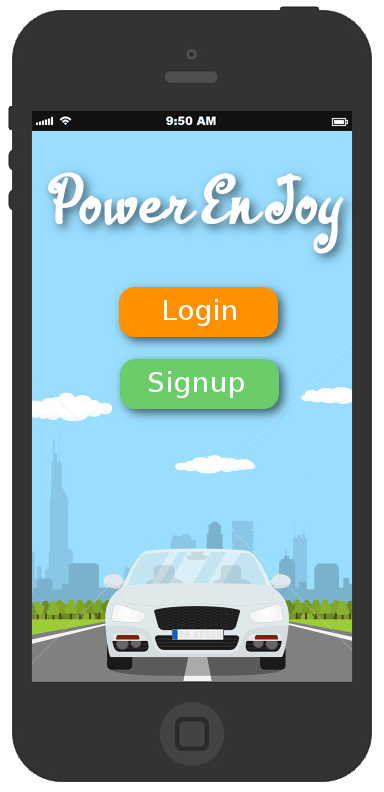
\includegraphics[width=0.2\textwidth]{mockup/1Login.png}
	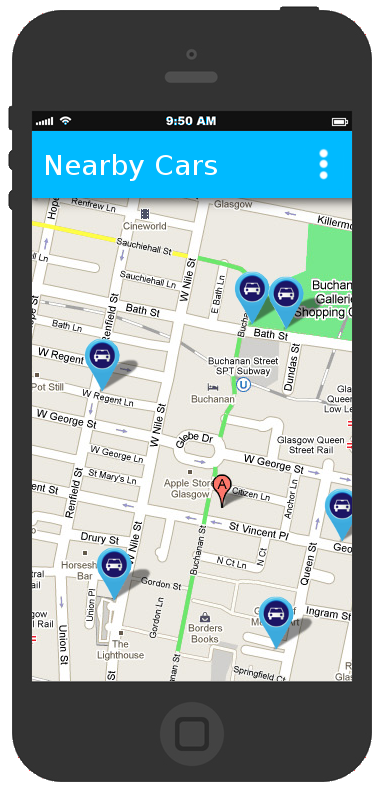
\includegraphics[width=0.2\textwidth]{mockup/2MainClient.png}
	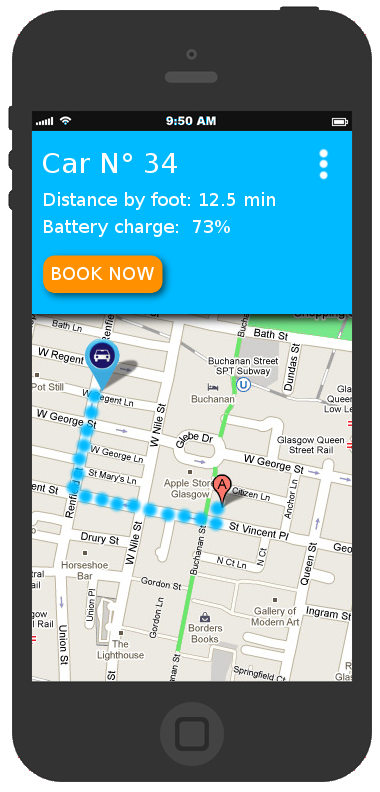
\includegraphics[width=0.2\textwidth]{mockup/3CarSelected.png}
	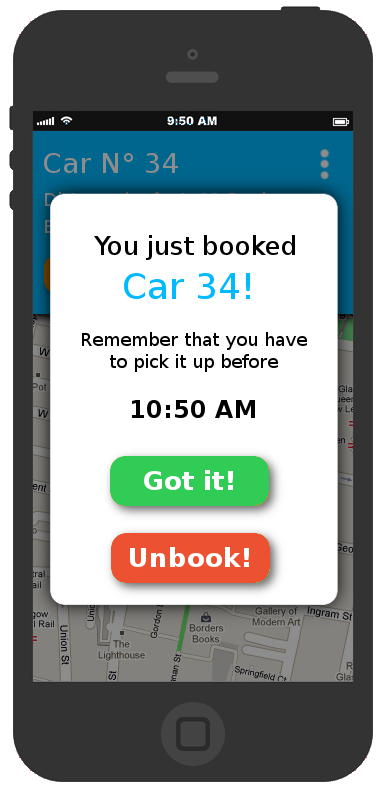
\includegraphics[width=0.2\textwidth]{mockup/4CarBooked.png}
	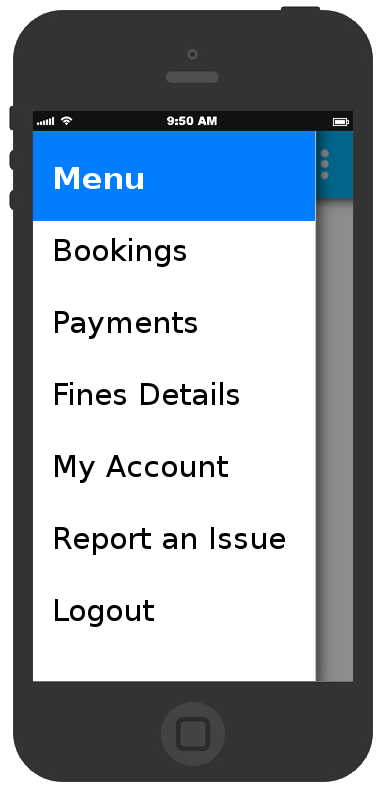
\includegraphics[width=0.2\textwidth]{mockup/11Menu.png}
	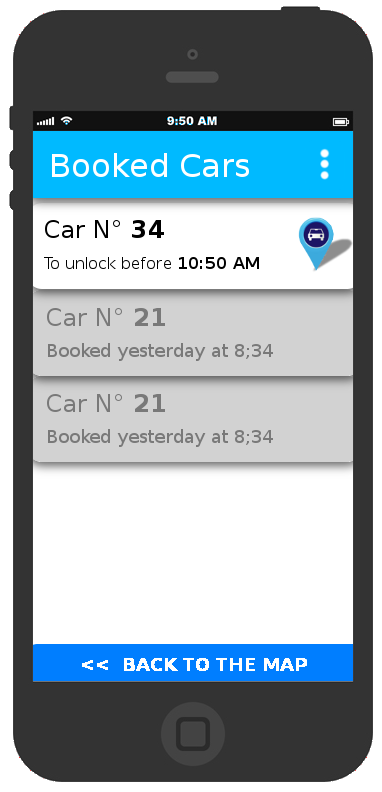
\includegraphics[width=0.2\textwidth]{mockup/5CarBookedList.png}
	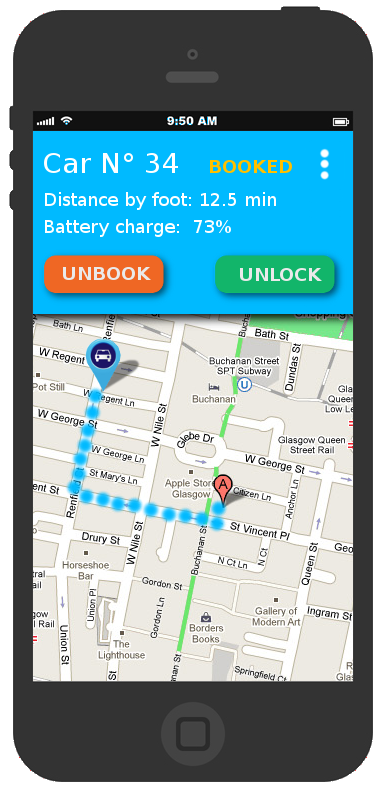
\includegraphics[width=0.2\textwidth]{mockup/6CarBookedSelected.png}
	%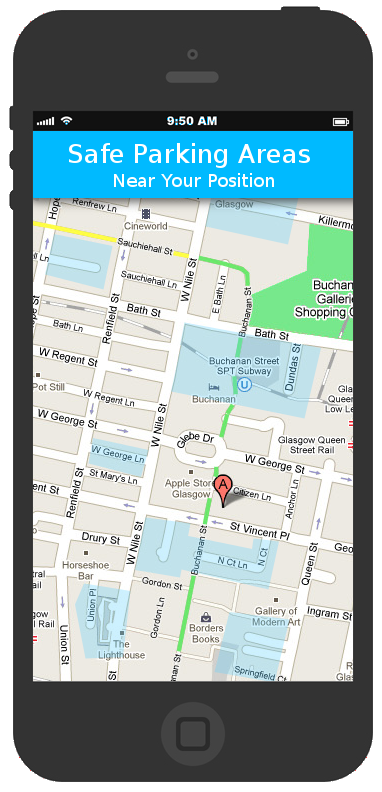
\includegraphics[width=0.2\textwidth]{mockup/7WhileDriving.png}
	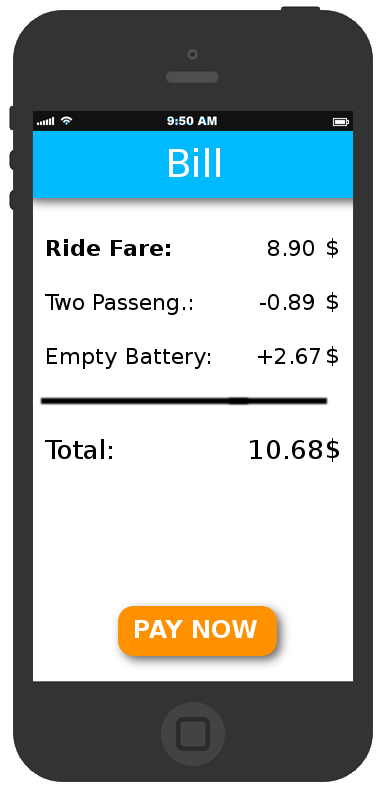
\includegraphics[width=0.2\textwidth]{mockup/8Bill.png} 	\hspace{0.8cm}
	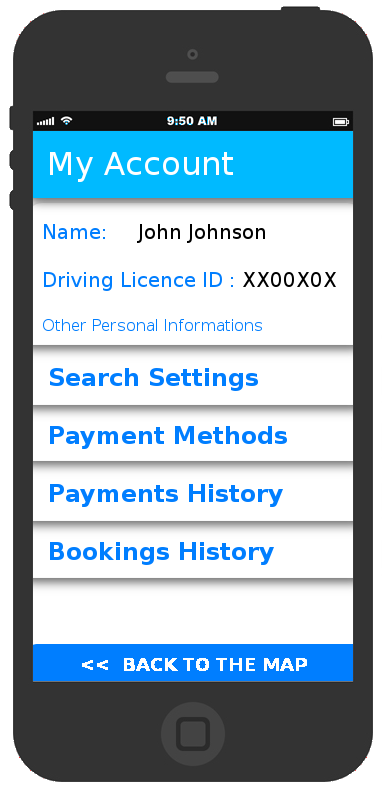
\includegraphics[width=0.2\textwidth]{mockup/9MyAccount.png} 	\hspace{0.8cm}
	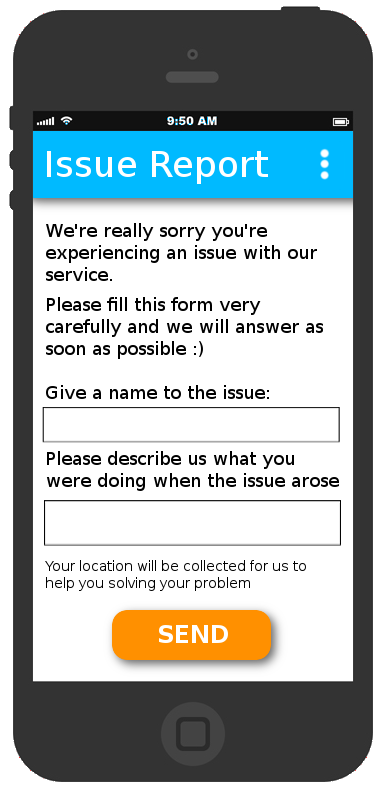
\includegraphics[width=0.2\textwidth]{mockup/12IssueReport.png} 	\hspace{0.8cm}
	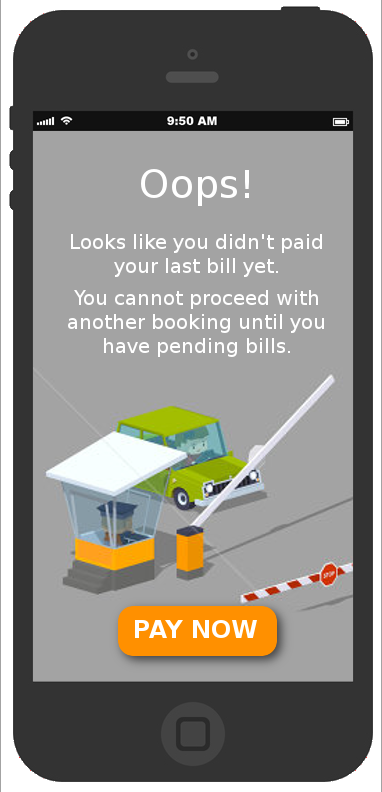
\includegraphics[width=0.2\textwidth]{mockup/10PendingBills.png} 	%\hspace{1cm}
	\caption{Mockup of the client's app main interfaces}
\end{figure}

\subsubsection{Car's Onboard System}
\begin{figure}[H]
	\centering
	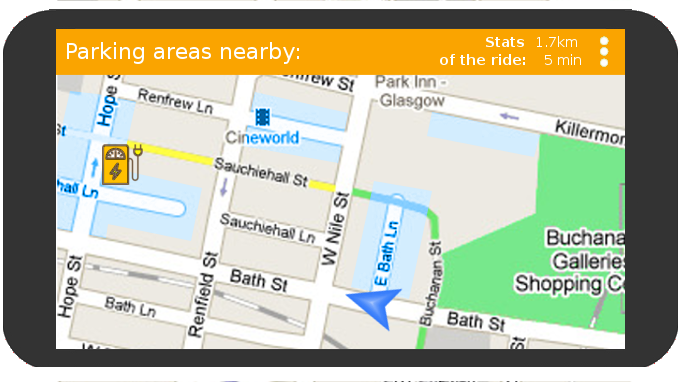
\includegraphics[width=0.6\textwidth]{mockup/CarsSystem} 
	\caption{Mockup of the car's onboard system as it should look while driving}
\end{figure}

\subsubsection{Staff's App Interface}
\begin{figure}[H]
	\centering
	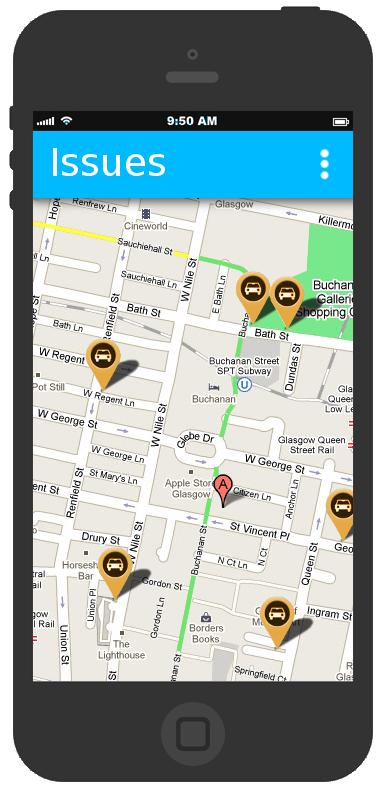
\includegraphics[width=0.2\textwidth]{mockup/AIssues.png} \hspace{0.8cm}
	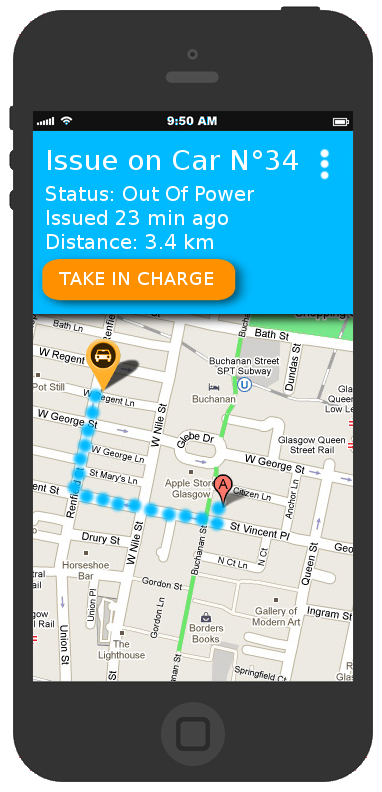
\includegraphics[width=0.2\textwidth]{mockup/BSelectedIssue.png} \hspace{0.8cm}
	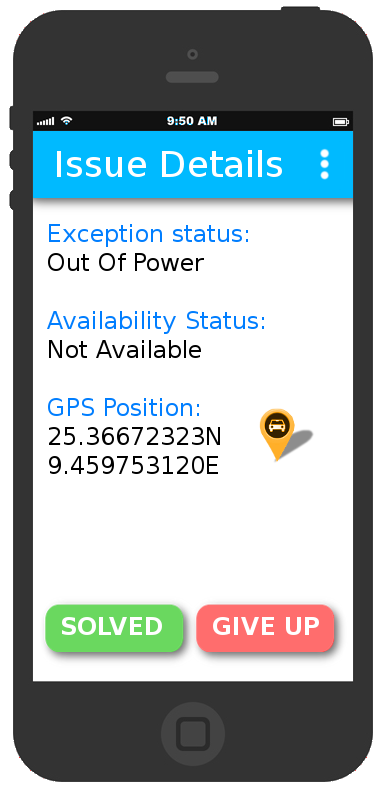
\includegraphics[width=0.2\textwidth]{mockup/CIssueDetail.png}
	\caption{Mockup of the staff's operators reserved interfaces}
\end{figure}
  

\newpage
\section{Scenarios, Use Cases and UML Diagrams}

\subsection{Scenarios}

\subsubsection{Scenario 1}
John has been abroad for a business trip, and now is at the airport, deciding how to go home. He is a user of \pecomma so  he opens the app and looks if there is any available car nearby. 

At the beginning the app tells him that, unfortunately, there are no available cars within ten minuted by foot; knowing the airport's parking is reachable in 10 minute by shuttle bus, he changes the settings to look for cars near a specific point on the map, and selects the airport's parking area. 

The app immediately finds many more cars: 6 with the battery almost fully charged and 2 with about half charge left. He chooses a random full charged car and reserves it; then takes his luggage, takes the shuttle bus and reach the car within 15 min. Once near the car, he presses the Unlock button on the car and the car unlocks. John can leave his luggage in the luggage van, enter the car and drive back home.

Once near home, John parks correctly the car in a safe area, as indicated by the car's onboard system. He exits the car, takes his luggage out and uses the app to lock the car, which has still 60\% of battery charge left. Once the lock is confirmed he receives the bill, calculated on the lenght and duration of the ride, and a 20\% discount as a bonus to have left the car with more than 50\% of battery charge. The nearest charging station locates within 3 km, so he gets no overprices.

John pays the bill immediately through the app.

\subsubsection{Scenario 2}
Anne want to go from his home to the airport to bring two friends home. Using \pe app she books the nearest car and within 10 minutes she started her ride to the airport.

Once near the destination, the car's onboard system tells her that there is a charging station nearby the airport. So Anne drives to the the charging station, parks, exits and plugs the car to the power grid. Then she locks the car. Once the lock is confirmed, she receives the bill and a 30\% discount as bonus for plugging the car to the grid.

While waiting for her friends, she reserves another car for coming back, but the plane is late and the reservation, which lasts one hour, expires. Anne receives a little penalty for the expired reservation and pays it immediately; then reserves again the car.

When her friends arrive, they all reach the car within 30 minutes from the second booking: they get on the car and drive to her friends' home. At arrival, the car has about 40\% of charge left, but there are no charging stations nearby (even if there is one at 2,1 km from their destination ), so Anne parks it in a safe area, exit, take luggages out and locks the car. The app sends her the bill and applies a 10\% discount as a bonus for bringing at least two friends on the same ride.


\subsubsection{Scenario 3}
Bob has an exam at 8 a.m., but the morning train is very late. So he decides to use \pe and go to the university by car. He looks for some cars near him, but he finds there is only one car left with about 40\% of residual charge. He reserves it anyways and within 5 minutes he started his ride to the university.

He is in a hurry, so drives very badly and commits some infractions, that gets recorded by the police. The policeman who is taking care of Bob's infractions looks in the police's databases for the owner of the car he spotted and sends the fine to \pe offices.

Once near his destination, the car's onboard system tells Bob that there is a charging station at about 10 minutes by foot from the university, and a parking area right in front of the entrance of the university. At the end of the ride, the car has only 15\% of residual charge.

Bob doesn't care and parks the car in front of the university, then exits and locks the car. The app confirms the lock and send him the bill, 30\% overpriced for having left the discharged car not plugged to the power grid, but at least he is in time for the exam.

Meanwhile at the company's offices, the fine is processed by a staff member and an email is sent to Bob's email address notifying him about the fine and the payment procedure he has to follow.


\subsubsection{Scenario 4}
It is a sunny Sunday and Charlie wants to go with his family in the countryside. He has no car, but he doesn't want to go there by train: so he decides to use \pe to do his trip. He finds a fully charged car near his house, reserves it and within 20 minutes he started his drive.

At the end of the day, Charlie wants to go back home with his family. He book the car he brought far from the city with him and shortly thereafter he starts his journey back home. He is halfaway from home when suddenly the car stops running: the engine got too much heat during the day and broke.

Charlie does not need to send a report to PowerEnJoy: the onboard system immediately tells him that an issue report has automatically been sent to the central. So Charlie receives the first part of the bill and, paid it, he can look for another car to finish his trip. He finds only one at half an hour by foot from his location. Charlie books the car and manages to reach it in time to unlock it and go back home.

When he arrives, he parks the car in a safe area near his house. He does not care about charging stations, because he saw that the car has about 80\% of charge; this way Charlie does not notice that the nearest charging station is at 4.3 km from the place he is parking the car.

He exits with all his family and locks the car: now he receives the bill, that is the basic price of the second ride, plus a 10\% discount for having brought many people on the car and a 30\% overprice for having left the car too far from a charging station.

Charlie tries to pay, but his payment fails because the rechargeable credit card he connected to the app has not enough money to pay the unexpected overprice. So he gets a notice from \pe that he is temporary banned from the service until he manages to pay the last pending bill.

\subsubsection{Scenario 5}
Harry is a staff operator of \pecomma in charge of re-chargin cars in-place when required. He has just completed another task, so he opens the app and looks for any other pending issues to solve.

The app gives him a list of issues near him: two discharged cars left far from a power station, one parked near a power station that needs to be plugged, a Technical Issue and a car parked outside from a safe area. Harry filters the issues based on their Exception status, in order to see only issues related to recharging, and gets a list of the three discharged cars. He takes in charge the nearest one pressing the button on his app's interface. The app shows him the way and Harry goes for that car.

Once near the car, Harry plugs the car to his portable charging station and charges it until it's almost full. Then changes manually the status of the car from Not Available to Available: but the system does not confirm the operation, because it cannot detect the residual charge of the battery. The Exception status of the car gets set to Mechanical Issue, but Harry has no means to fix that problem: so he does not take charge of the new issue and goes for another car to charge.


\subsection{Use Cases}

\subsubsection{Use Case Diagram}
\begin{figure}[H]
	\centering
	\includegraphics[width=0.8\textwidth]{UML/UseCaseDiagram.png}
	\caption{Use Case Diagram for Customers and Staff Operators}
\end{figure}

\subsubsection{Customer's Use Cases Description}

\begin{description}[noitemsep,topsep=0pt,parsep=0pt,partopsep=0pt]
	\item[Name:] \textbf{Register}
	\item[Actors Involved:] A future user.
	\item[Entry Conditions:] None
	\item[Flow Of Events:] \hfill\
	\begin{itemize}
		\item Opens the app, presses the Register button
		\item Fills the form with their personal information including a chosen password, Driving Licence Informations and payment informations.
		\item Confirms they took vision of Terms and Conditions of the Service 
		\item Can press the Confirm button.
	\end{itemize} \hfill\
	\item[Exit conditions:] The customer is successfully redirected to the Login page.
	\item[Exceptions:]  \hfill\
	\begin{itemize}
		\item The user filled the form with invalid data: the app redirects him back to the form and highlights recognized problems. 
		\item The user is found to have another account already active: they are redirected to the Login page with a notice that states they must login with their original credentials.
	\end{itemize}
\end{description}
\hfill\


\begin{description}[noitemsep,topsep=0pt,parsep=0pt,partopsep=0pt]
	\item[Name:] \textbf{Login}
	\item[Actors Involved:] A registered user.
	\item[Entry Conditions:] None
	\item[Flow Of Events:]  \hfill\
	\begin{itemize}
		\item Open the app, presses the Login button
		\item Fill the form with their username - password pair.
		\item Press the Login button.
	\end{itemize}
	\item[Exit conditions:] The customer is successfully redirected to the Cars Nearby page.
	\item[Exceptions:]  \hfill\
	\begin{itemize}
		\item The user inputs a wrong username - password pair: they are redirected back to the Login page with a notice. 
	\end{itemize}
\end{description}
\hfill\

\begin{description}[noitemsep,topsep=0pt,parsep=0pt,partopsep=0pt]
	\item[Name:] \textbf{Book cars}
	\item[Actors Involved:] A registered user, a car.
	\item[Entry Conditions:] The user logged in and have no pending bills to pay.
	\item[Flow Of Events:]  \hfill\
	\begin{itemize}
		\item Look at the Cars Nearby page and choses the car they want to book.
		\item Click on the car they chosed and see additional informations.
		\item Click the Book button.
		\item The system changes the status of the car from Available to Booked.
	\end{itemize}
	\item[Exit conditions:] The customer receives a notification confirming the operation, and see the deadline to unlock the car.
	\item[Exceptions:] No predictable exceptions at this stage.
\end{description}
\hfill\

\begin{description}[noitemsep,topsep=0pt,parsep=0pt,partopsep=0pt]
	\item[Name:] \textbf{Unbook cars}
	\item[Actors Involved:] A user who booked a car, the booked car.
	\item[Entry Conditions:] The user logged in and has booked a car, but not yet unlocked it.
	\item[Flow Of Events:] \hfill\
	\begin{itemize}
		\item Press the Menu icon in the top-right corner of the screen.
		\item Press Bookings to see the bookings history.
		\item Select the active booking they want to quit.
		\item They receive a confirmation notice.
		\item Press the Unbook button.
		\item The system changes the status of the car from Booked to Available.
	\end{itemize}
	\item[Exit conditions:] The customer receives a notification confirming the operation.
	\item[Exceptions:] No predictable exceptions at this stage.
\end{description}
\hfill\

\begin{description}[noitemsep,topsep=0pt,parsep=0pt,partopsep=0pt]
	\item[Name:] \textbf{Unlock booked cars}
	\item[Actors Involved:] A user who booked a car, the booked car.
	\item[Entry Conditions:] The user logged in and has booked a car, but not yet unlocked it.
	\item[Flow Of Events:] \hfill\
	\begin{itemize}
		\item Press the Unlock button on the Booking Page of the app.
		\item The system unlocks the car.
		\item The system changes the status of the car from Booked to Unlocked.
	\end{itemize}
	\item[Exit conditions:]  The user receives a notification their car has been unlocked.
	\item[Exceptions:] \hfill\
	\begin{itemize}
		\item The car doesn't unlock: the user can send again the unlock request pressing again the button.
	\end{itemize}
\end{description}
\hfill\

\begin{description}[noitemsep,topsep=0pt,parsep=0pt,partopsep=0pt]
	\item[Name:] \textbf{Drive unlocked cars}
	\item[Actors Involved:] A user who unlocked a car, the unlocked car.
	\item[Entry Conditions:] The user logged in and has unlocked its car.
	\item[Flow Of Events:] \hfill\
	\begin{itemize}
		\item Enter the unlocked car.
		\item Scan their driving licence.
		\item Receive a confirmation the scanned driving licence matches.
		\item Switch on the car and drive to the destination.
		\item The system changes the status of the car from Unlocked to Running
	\end{itemize}
	\item[Exit conditions:]  The user receives a notification their driving time has begun.
	\item[Exceptions:] \hfill\
	\begin{itemize}
		\item The scanned driving licence is not correct for the user who booked the car: a notice is sent to the user and a new scan is expected.
	\end{itemize}
\end{description}
\hfill\

\begin{description}[noitemsep,topsep=0pt,parsep=0pt,partopsep=0pt]
	\item[Name:] \textbf{Parks safely and charge the car}
	\item[Actors Involved:]  A user that is driving a car, the car itself.
	\item[Entry Conditions:] The user is driving a car.
	\item[Flow Of Events:] \hfill\
	\begin{itemize}
		\item See the location of safe areas and charging stations on the map.
		\item Park in a safe location and switch off the engine.
		\item The system sees this change and sets the status of the car from Running to Parked.
		\item If near to a charging station, the driver may plug the car to the power grid.
		\item Confirm the parking pressing the Lock button.
		\item The system locks the car.
		\item The system changes the status of the car from Parked to Available.
	\end{itemize}
	\item[Exit conditions:]  The user receives a confirmation the car has been locked.
	\item[Exceptions:] \hfill\
	\begin{itemize}
		\item The car's engine stops out from a safe area: the user is notified and, if they leave, fined.
	\end{itemize}
\end{description}
\hfill\

\begin{description}[noitemsep,topsep=0pt,parsep=0pt,partopsep=0pt]
	\item[Name:] \textbf{Pay bills and get discounts for virtuous behavior}
	\item[Actors Involved:] A user who just finished a ride.
	\item[Entry Conditions:] The user locked a car after a ride.
	\item[Flow Of Events:] \hfill\
	\begin{itemize}
		\item Receives the bill, including the regular fare plus eventual discounts or overprices for their behavior.
		\item Press the Pay Now button at the bottom of the bill.
		\item Pay the fee.
	\end{itemize}
	\item[Exit conditions:]  The user receives a confirmation that the payment has been completed successfully.
	\item[Exceptions:] \hfill\
	\begin{itemize}
		\item The payment fails: all the app's functions are locked until the user manages to pay the pending bill.
	\end{itemize}
\end{description}
\hfill\

\begin{description}[noitemsep,topsep=0pt,parsep=0pt,partopsep=0pt]
	\item[Name:] \textbf{Report an issue}
	\item[Actors Involved:]  A user who is experiencing an issue.
	\item[Entry Conditions:] The user notices something wrong with the app or the car.
	\item[Flow Of Events:] \hfill\
	\begin{itemize}
		\item Press the button Report An Issue.
		\item Fill the form and describe the issue.
		\item Send the Issue Report.
	\end{itemize}
	\item[Exit conditions:]  The user receives a confirmation that their report has been sent successfully.
	\item[Exceptions:] No predictable issue can happen at this stage.
\end{description}
\hfill\

\subsubsection{Staff Operator's Use Cases Description}

\begin{description}[noitemsep,topsep=0pt,parsep=0pt,partopsep=0pt]
	\item[Name:] \textbf{Take issue in charge}
	\item[Actors Involved:] An operator.
	\item[Entry Conditions:] The operator is logged in.
	\item[Flow Of Events:] \hfill\
	\begin{itemize}
		\item Looks at the map showing the nearest issues.
		\item Select a issue tapping on it.
		\item Press the Take in Charge button.
	\end{itemize}
	\item[Exit conditions:]  The user receives a confirmation that they took that issue in charge and receive directions to reach the involved vehicle.
	\item[Exceptions:] No predictable issue can happen at this stage.
\end{description}
\hfill\

\begin{description}[noitemsep,topsep=0pt,parsep=0pt,partopsep=0pt]
	\item[Name:] \textbf{Unlock car taken in charge}
	\item[Actors Involved:] An operator who took an issue in charge, the car with the issue considered.
	\item[Entry Conditions:] The operator is logged in and took an issue in charge.
	\item[Flow Of Events:] \hfill\
	\begin{itemize}
		\item Press the Unlock button on the app's interface.
		\item The system unlocks the selected car.
	\end{itemize}
	\item[Exit conditions:]  The car gets unlocked.
	\item[Exceptions:] \hfill\
	\begin{itemize}
		\item The car doesn't unlock: the operator can unlock it pressing the button again or give up the issue.
	\end{itemize}
\end{description}
\hfill\

\begin{description}[noitemsep,topsep=0pt,parsep=0pt,partopsep=0pt]
	\item[Name:] \textbf{Mark an issue as solved or give up an issue}
	\item[Actors Involved:] An operator who took an issue in charge, the car with the issue considered.
	\item[Entry Conditions:] The operator is logged in and took an issue in charge.
	\item[Flow Of Events:] \hfill\
	\begin{itemize}
		\item Open the Issue page, stating more details about the issue taken in charge.
		\item Press the Solved button if enabled, or
		\item Press the Give Up button.
		\item The system reacts to the solution either checking the car's availability or locking it back for another operator to take it in charge.
	\end{itemize}
	\item[Exit conditions:]  The operator receives a notice confirming the operation.
	\item[Exceptions:]  \hfill\
	\begin{itemize}
		\item The system doesn't confirm the issue has been solved: the issue status is changed to Technical issue and nother, different issue is generated.
	\end{itemize}
\end{description}
\hfill\

\begin{description}[noitemsep,topsep=0pt,parsep=0pt,partopsep=0pt]
	\item[Name:] \textbf{Change car's Exception status}
	\item[Actors Involved:] An operator who took an issue in charge, the car with the issue considered.
	\item[Entry Conditions:] The operator is logged in and took an issue in charge.
	\item[Flow Of Events:] \hfill\
	\begin{itemize}
		\item Open the Issue page, stating more details about the issue taken in charge.
		\item Changes the Exception status choosing an item from the list.
		\item Press the Confirm button.
	\end{itemize}
	\item[Exit conditions:]  The operator receives a notice confirming the operation.
	\item[Exceptions:] No predictable exception at this stage.
\end{description}
\hfill\

\begin{description}[noitemsep,topsep=0pt,parsep=0pt,partopsep=0pt]
	\item[Name:] \textbf{Find out who was driving a car in a specificed moment}
	\item[Actors Involved:] An operator.
	\item[Entry Conditions:] The operator is logged in.
	\item[Flow Of Events:] \hfill\
	\begin{itemize}
		\item Open the Find Driver page.
		\item Input the car details and the time of the supposed ride, or can select the "Last Driver" option to find the last user who drove that car.
		\item Press the button Contact the Driver.
	\end{itemize}
	\item[Exit conditions:]  The operator can contact the user who was driving that car in that specified moment.
	\item[Exceptions:] \hfill\
	\begin{itemize}
		\item The operator input invalid data: they are redirected back to the form page, highlighting the problem.
		\item The car was parked in the specified moment: the operator is told there is no driver related to that car in that moment.
	\end{itemize}
\end{description}
\hfill\

\subsection{Other UML Diagrams}

\subsubsection{Sequence Diagrams}
\begin{figure}[H]
	\centering
	\includegraphics[width=1\textwidth]{UML/SequenceDiagramLoginReg.png}
	\caption{Registration and Login Process}
\end{figure}
\begin{figure}[H]
	\centering
	\includegraphics[width=1\textwidth]{UML/SequenceDiagramBooking.png}
	\caption{Booking Process}
\end{figure}
\begin{figure}[H]
	\centering
	\includegraphics[width=1\textwidth]{UML/SequenceDiagramPaying.png}
	\caption{Locking and Paying Process}
\end{figure}
\begin{figure}[H]
	\centering
	\includegraphics[width=0.8\textwidth]{UML/SequenceDiagramIssue.png}
	\caption{Issues Management Process}
\end{figure}

\subsubsection{Activity Diagrams}
\begin{figure}[H]
	\centering
	\includegraphics[width=0.6\textwidth]{UML/ActivityBooking.png}
	\caption{Booking Flow}
\end{figure}

\begin{figure}[H]
	\centering
	\includegraphics[width=0.6\textwidth]{UML/ActivityIssue.png}
	\caption{Issue Management Flow}
\end{figure}
\newpage


\subsubsection{State Diagrams}
\begin{figure}[H]
	\centering
	\includegraphics[width=0.8\textwidth]{UML/StateDiagramCarAvailability.png}
	\caption{Car's Availability Status State Transitions}
\end{figure}
\begin{figure}[H]
	\centering
	\includegraphics[width=0.8\textwidth]{UML/StateDiagramIssues.png}
	\caption{Issue's State Transitions}
\end{figure}



\newpage
\section{Alloy Model}

To check the validity of the proposed solution we implemented a model in Alloy.

In order to keep the model itself manageable, it was first developed in small chucks and their validity checked. Then each chuck has been merged in a bigger model and the validity of the resulting model has been re-check again.

\begin{figure}[H]
	\centering
	\includegraphics[width=1\textwidth]{UML/ClassDiagram.png}
	\caption{Class Diagram for the Alloy Model}
\end{figure}

\subsection{Main Model}

\lstinputlisting[language=alloy]{Alloy/COMPLETE.als}

\subsubsection{Results of Execution}

\begin{figure}[H]
	\centering
	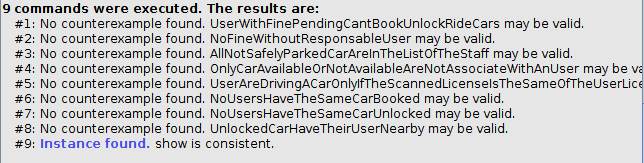
\includegraphics[width=0.8\textwidth]{Alloy/ConsistentStatic.png}
	\caption{Output of the Alloy Analizer}
\end{figure}

\subsubsection{Generated graph}

\begin{figure}[H]
	\centering
	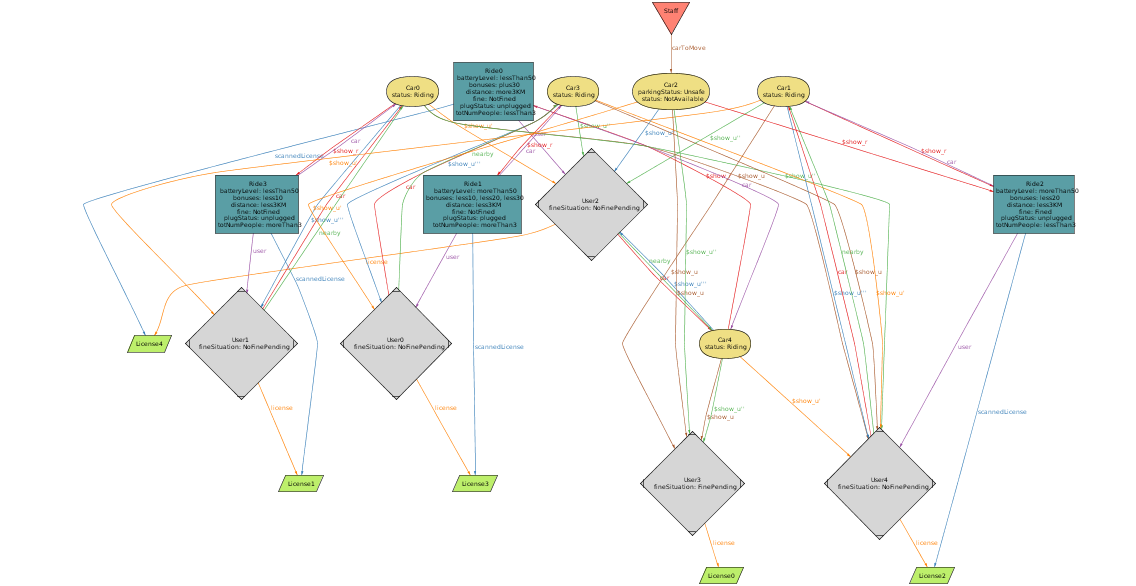
\includegraphics[width=1\textwidth]{Alloy/Complete.png}
	\caption{One of the model returned by Alloy, compressed visualization}
\end{figure}

\subsection{Dynamic Model}

Finally, in order to check the validity of our solution in a dynamic context, we develop another smaller Alloy model of the dynamic aspects of the system.

\subsubsection{Model}
\lstinputlisting[language=alloy]{Alloy/BOOK_DYNAMIC.als}

\subsubsection{Result of Execution}
\begin{figure}[H]
	\centering
	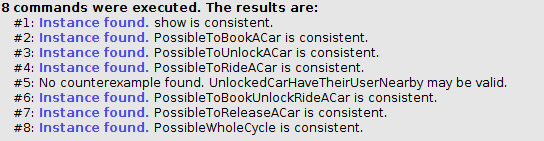
\includegraphics[width=0.8\textwidth]{Alloy/DynamicConsistent.png}
	\caption{Output of the Alloy Analizer}
\end{figure}

\newpage
\section{Conclusions}

\subsection{Future Development}
There are a lot of aspects of \pe that can be improved in the future.

For example, users may show the need to exit their car for a short amount of time during the ride: for example, to go shopping and then come back home. This can be an improvement in the next versions of the software.

We may also think at more bonuses for virtuous behaviours that at this stage were not considered: for example, leaving the car in an area where there are on average a lot of requests can be seen as a virtuous behavior that can be rewarded.

We can also think at different payment methods for frequent users, like prepaid credit related to user's account, or discounts for very frequent (i.e. daily) and usually virtuous users of the service.

\subsection{Tools used}
During the development of this document we used the following tools:
\begin{itemize}
	\item \textbf{Github} to version control the project
	\item \textbf{\LaTeX} on TeXworks to redact this document
	\item \textbf{Alloy Analyzer v.4.2} to check model's validity
	\item \textbf{www.draw.io} to draw UML graphs
	\item \textbf{Gimp v.2.8} to mockup the application
\end{itemize}

\subsection{Hours of work}

\begin{itemize}
	\item SZ: 4h on 1/11
	\item SZ: 4h on 4/11
	\item SM: 5h on 4/11
	\item SZ: 6h on 5/11
	\item SM: 2h on 6/11
	\item SM: 4h on 7/11
	\item SZ: 4h on 7/11
	\item SM: 4h on 9/11
	\item SZ: 2h on 10/11
	\item SM: 4h on 10/11
	\item SZ: 2h on 11/11
	\item SZ: 4h on 12/11
	\item SM: 6h on 12/11
\end{itemize}

\subsection{Changelog}
\begin{itemize}
	
	\item v 1.1

	Fix missing UNBOOK requirement and related minor fixes.
	\begin{itemize}
		\item ADD the sentence ``or five minutes after the car is unblocked.'' on subsection 2.7, ``Assumptions on the car system'', point 10.
		\item ADD requirement ``UNBOOK''.
		\item UPDATE 5th point at page 11, ``The Availability status can change to Available only if it was \textit{Booked}, Parked or Not Available.
	\end{itemize}
	
	\item v 1.2
	
	Clarify and review fines management and fix the unlocking procedure.
	\begin{itemize}
		\item ADD paragraph ``Fines`` at page 6
		\item UPDATE ``FINES`` goal under section 3.1:Goals, page 14
		\item UPDATE ``FINES`` requirements under section 3.2: Functional Requirements, page 19
		\item UPDATE Scenario 3 under section 4.1: Scenarios, page 23
		\item UPDATE Use Case Diagram Figure (Figure 4, page 25) and the last Use Case description, replacing it with a new one, ``Find out who was driving a car in a specified moment``, page 30.
		\item UPDATE ``UNLOCK`` requirements under section 3.2: Functional Requirements, page 16
		\item UPDATE a Use Case related to the unlocking procedure under section 4.2: Use Cases
	\end{itemize}

	\item v 1.3
	\begin{itemize}
		\item UPDATE goal ``LOOKUP`` to better specify it.
		\item ADD REPORT\_ISSUE goal and REP1, REP2 as related requirements.
	\end{itemize}	
	
	\item v 1.4
	\begin{itemize}
		\item UPDATE Alloy adding check fot tge ``UNBOOK'' requirement.
	\end{itemize}

\end{itemize}

\end{document}
